\documentclass{article}
\usepackage[utf8]{inputenc}
\usepackage[a4paper, margin=1in]{geometry}
\usepackage{siunitx}
\usepackage{amsmath}
\usepackage{enumitem}
\usepackage{esdiff}
\usepackage{pgfplots}
\usepackage{listings}
\usepackage{xcolor}
\usepackage{amssymb}

\pgfplotsset{compat=1.18, width=10cm}

\tolerance=1
\emergencystretch=\maxdimen
\hyphenpenalty=10000
\hbadness=10000

\sisetup{
    input-ignore={.},
    output-decimal-marker={,},
    group-minimum-digits=4,
    group-separator={.},
    group-digits=integer
}

\definecolor{darkgray}{rgb}{.4,.4,.4}

\lstdefinestyle{code}{
    aboveskip={1.3\baselineskip},
    basicstyle=\scriptsize\ttfamily\linespread{4},
    breaklines=false,
    columns=fullflexible,
    commentstyle=\color[rgb]{0.127,0.427,0.514}\ttfamily\itshape,
    escapechar=@,
    extendedchars=true,
    frame=single,
    identifierstyle=\color{black},
    inputencoding=latin1,
    keywordstyle=\color[HTML]{228B22}\bfseries,
    ndkeywordstyle=\color[HTML]{228B22}\bfseries,
    numbers=left,
    numberstyle=\tiny,
    prebreak = \raisebox{0ex}[0ex][0ex]{\ensuremath{\hookleftarrow}},
    stringstyle=\color[rgb]{0.639,0.082,0.082}\ttfamily,
    upquote=true,
    showstringspaces=false,
    xleftmargin=5ex,
    aboveskip=5pt
}

\newcommand{\penyelesaian}{\textbf{Penyelesaian: }}

\title{\textbf{Komputasi Numerik: Tugas 2}}
\author{Kelompok 15}
\date{}

\begin{document}

\maketitle

\begin{enumerate}
    \item Dengan metode grafik, dapatkan akar-akar persamaan:
    \begin{enumerate}
        \item $e^x - x - 2 = 0$ \\
        \penyelesaian $e^x - x - 2 = 0 \Leftrightarrow e^x = x + 2$, sehingga diperoleh dua persamaan $y = e^x$ dan $y = x + 2$. 
        Grafik dari kedua persamaan tersebut diperoleh sebagai berikut.
        \begin{center}
            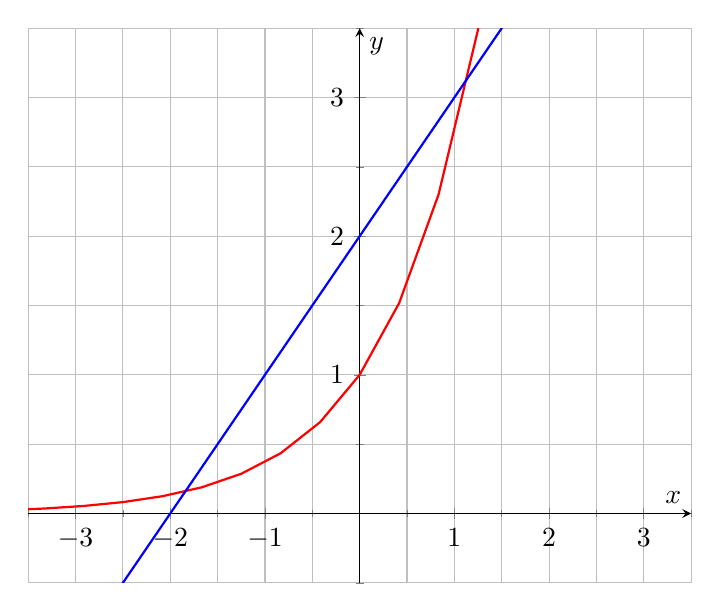
\begin{tikzpicture}
                \begin{axis}[grid=both,ymin=-0.5,ymax=3.5,xmax=3.5,xmin=-3.5,
                             minor tick num=1,axis lines = middle,xlabel=$x$,ylabel=$y$]
                    \addplot[color=red, thick]{e^x};
                    \addplot[color=blue, thick]{x+2};
                \end{axis}
            \end{tikzpicture}
        \end{center}
        Berdasarkan letak perpotongan garis dari dua persamaan, diperoleh dua akar, yakni $x_1$ yang terletak di antara $(-2, 1)$ dan $x_2$ yang terletak di antara $(1, 2)$.

        \item $10^x = 100 - 2x$ \\
        \penyelesaian Diperoleh dua persamaan, $y = 10^x$ dan $y = 100 - 2x$. Berikut hasil plot dari kedua persamaan tersebut.
        \begin{center}
            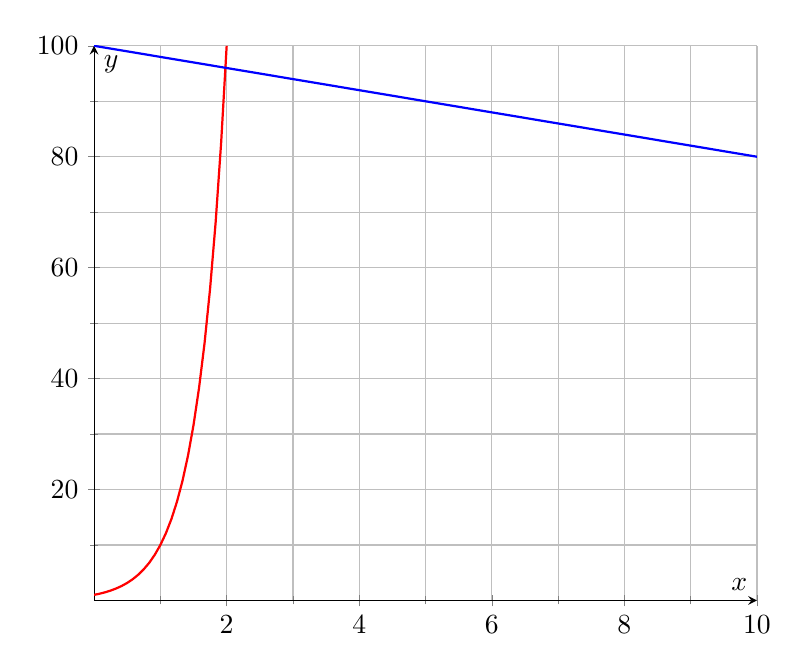
\begin{tikzpicture}
                \begin{axis}[grid=both,ymin=0,ymax=100,xmax=10,xmin=0,
                             minor tick num=1,axis lines = middle,xlabel=$x$,ylabel=$y$]
                    \addplot[red, thick, domain=0:2]{10^x};
                    \addplot[color=blue, thick, domain=0:10]{100-2*x};
                \end{axis}
            \end{tikzpicture}
        \end{center}
        Berdasarkan letak perpotongan dua garis, diperoleh informasi bahwa fungsi hanya memiliki satu akar $x$.

        Grafik diperbesar pada akar $x$:
        \begin{center}
            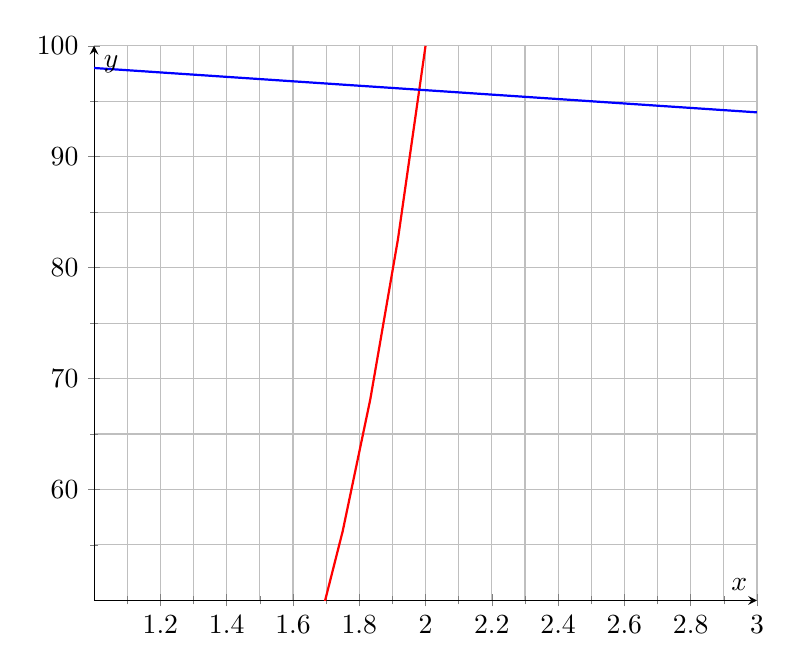
\begin{tikzpicture}
                \begin{axis}[grid=both,ymin=50,ymax=100,xmax=3,xmin=1,
                             minor tick num=1,axis lines = middle,xlabel=$x$,ylabel=$y$]
                    \addplot[red, thick, domain=0:2]{10^x};
                    \addplot[color=blue, thick, domain=0:10]{100-2*x};
                \end{axis}
            \end{tikzpicture}
        \end{center}
        Dengan demikian, akar $x$ dapat dipastikan berada di sekitar $(\num{1,9}; \num{2,0})$.

        \item $\num{-0,874}x^2 + \num{1,75}x + \num{2,627}$ \\
        \penyelesaian $y = \num{-0,874}x^2 + \num{1,75}x + \num{2,627}$, untuk mencari akar-akar persamaan maka $y = 0$. \\

        $\num{-0,874}x^2 + \num{1,75}x + \num{2,627} = 0 \Leftrightarrow \num{0,874}x^2 = \num{1,75}x + \num{2,627}$, diperoleh dua persamaan, $y = \num{0,874}x^2$ dan $y = \num{1,75}x + \num{2,627}$.
        Grafik dari kedua persamaan tersebut diperoleh sebagai berikut.
        \begin{center}
            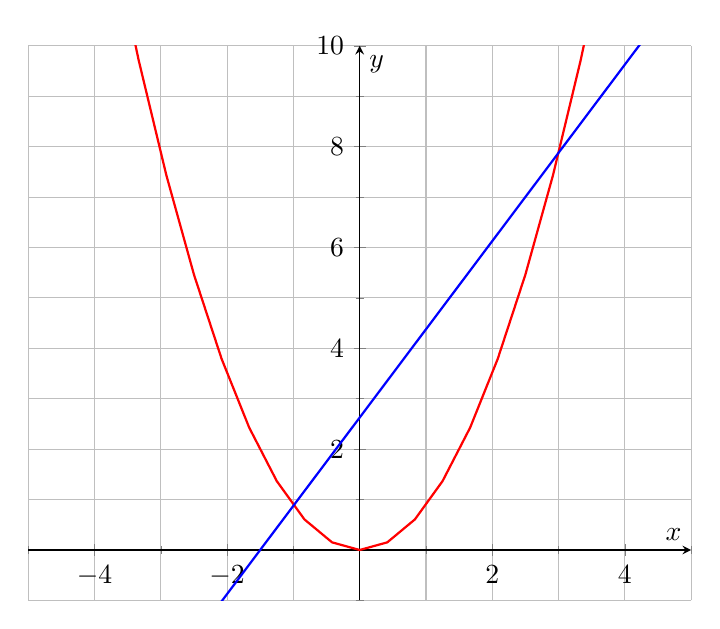
\begin{tikzpicture}
                \begin{axis}[grid=both,ymin=-1,ymax=10,xmax=5,xmin=-5,
                             minor tick num=1,axis lines = middle,xlabel=$x$,ylabel=$y$]
                    \addplot[color=red, thick]{0.874*x^2};
                    \addplot[color=blue, thick]{1.75*x + 2.627};
                \end{axis}
            \end{tikzpicture}
        \end{center}
        Berdasarkan letak perpotongan garis, diperoleh dua akar, yaitu $x_1$ dan $x_2$.\\

        Grafik diperbesar pada titik $x_1$:
        \begin{center}
            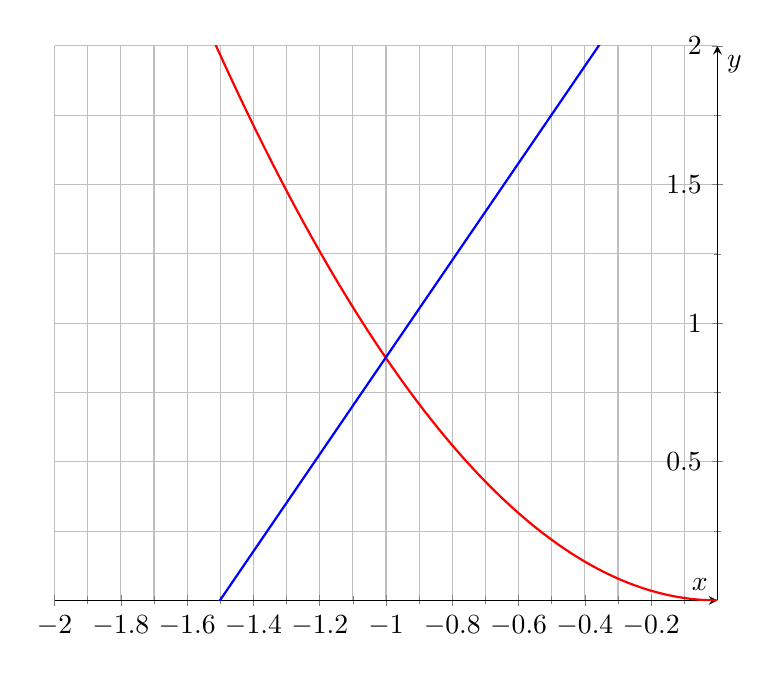
\begin{tikzpicture}
                \begin{axis}[grid=both,ymin=0,ymax=2,xmax=0,xmin=-2,samples=200,
                             minor tick num=1,axis lines = middle,xlabel=$x$,ylabel=$y$]
                    \addplot[color=red, thick, domain=-2:0]{0.874*x^2};
                    \addplot[color=blue, thick, domain=-2:0]{1.75*x + 2.627};
                \end{axis}
            \end{tikzpicture}
        \end{center}

        Grafik diperbesar pada titik $x_2$:
        \begin{center}
            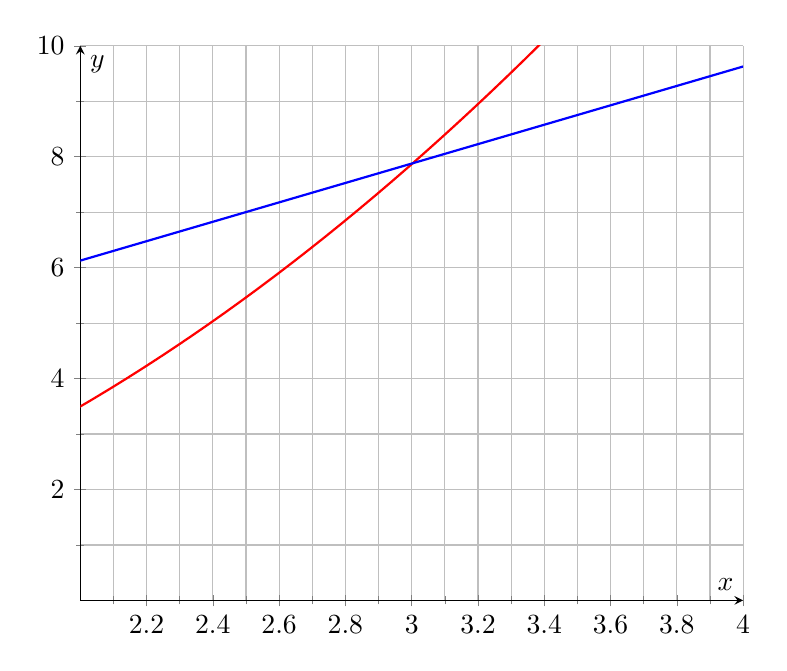
\begin{tikzpicture}
                \begin{axis}[grid=both,ymin=0,ymax=10,xmax=4,xmin=2,samples=200,
                             minor tick num=1,axis lines = middle,xlabel=$x$,ylabel=$y$]
                    \addplot[color=red, thick]{0.874*x^2};
                    \addplot[color=blue, thick]{1.75*x + 2.627};
                \end{axis}
            \end{tikzpicture}
        \end{center}
        Dengan demikian, akar $x_1$ dapat dipastikan terletak di sekitar $(\num{-1,1}; \num{-1,0})$ dan $x_2$ dapat dipastikan terletak di sekitar $(\num{3,0}; \num{3,1})$

        \item $\num{-2,1} + \num{6,21}x - \num{3,9}x^2 + \num{0,667}x^3$ \\
        \penyelesaian $y = \num{-2,1} + \num{6,21}x - \num{3,9}x^2 + \num{0,667}x^3$, \\
        $y = 0 \implies \num{-2,1} + \num{6,21}x - \num{3,9}x^2 + \num{0,667}x^3 = 0 \Leftrightarrow \num{2,1} + \num{3,9}x^2 = \num{6,21}x + \num{0,667}x^3$.
        Diperoleh dua persamaan, $y = \num{2,1} + \num{3,9}x^2$ dan $y = \num{6,21}x + \num{0,667}x^3$. \\

        Grafik dari kedua persamaan tersebut diperoleh sebagai berikut.
        \begin{center}
            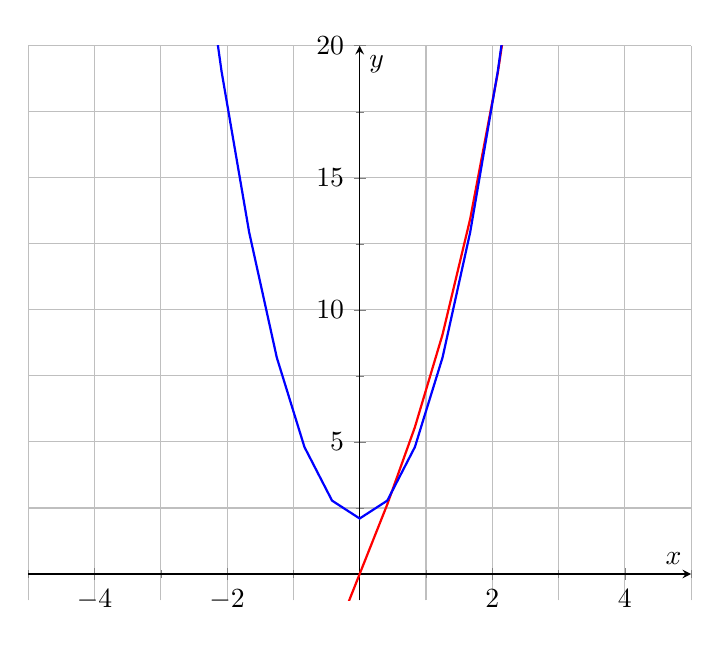
\begin{tikzpicture}
                \begin{axis}[grid=both,ymin=-1,ymax=20,xmax=5,xmin=-5,
                             minor tick num=1,axis lines = middle,xlabel=$x$,ylabel=$y$]
                    \addplot[color=red, thick]{6.21*x + 0.667*x^3};
                    \addplot[color=blue, thick]{2.1 + 3.9*x^2};
                \end{axis}
            \end{tikzpicture}
        \end{center}
        Terlihat bahwa kedua persamaan berpotongan di dua titik berbeda, yaitu $x_1$ dan $x_2$. 
        Kita dapat perbesar grafik di kedua titik tersebut agar dapat melihat informasi yang lebih jelas dari akar-akar persamaannya.\\

        Grafik diperbesar pada titik $x_1$:
        \begin{center}
            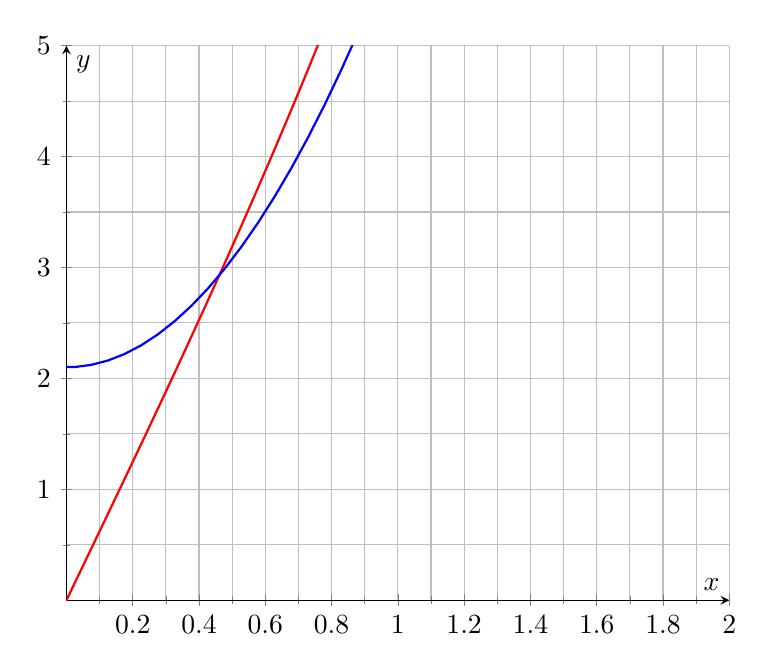
\begin{tikzpicture}
                \begin{axis}[grid=both,ymin=0,ymax=5,xmax=2,xmin=0,samples=200,
                             minor tick num=1,axis lines = middle,xlabel=$x$,ylabel=$y$]
                    \addplot[color=red, thick]{6.21*x + 0.667*x^3};
                    \addplot[color=blue, thick]{2.1 + 3.9*x^2};
                \end{axis}
            \end{tikzpicture}
        \end{center}

        Grafik diperbesar pada titik $x_2$:
        \begin{center}
            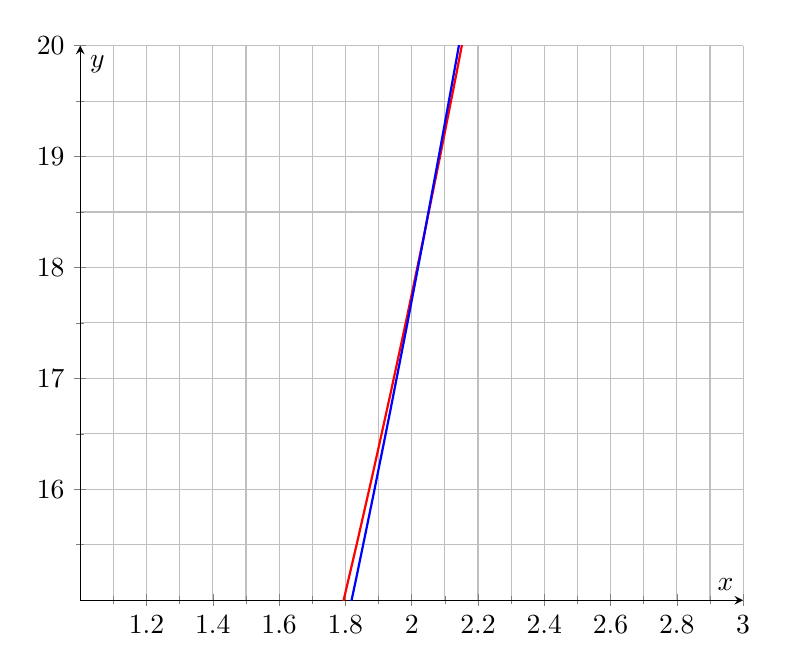
\begin{tikzpicture}
                \begin{axis}[grid=both,ymin=15,ymax=20,xmax=3,xmin=1,samples=200,
                             minor tick num=1,axis lines = middle,xlabel=$x$,ylabel=$y$]
                    \addplot[color=red, thick]{6.21*x + 0.667*x^3};
                    \addplot[color=blue, thick]{2.1 + 3.9*x^2};
                \end{axis}
            \end{tikzpicture}
        \end{center}
        Dengan demikian, dapat dipastikan $x_1$ terletak di sekitar $(\num{0,4}; \num{0,5})$ dan $x_2$ terletak di sekitar $(\num{2,0}; \num{2,1})$.

        \item $(1 - \num{0,6}x)/x$ \\
        \penyelesaian $y = (1 - \num{0,6}x)/x = 1/x - \num{0,6}$, sehingga diperoleh dua persamaan, yaitu $y = 1/x$ dan $y = \num{0,6}$.
        Grafik dari kedua persamaan tersebut diperoleh sebagai berikut.
        \begin{center}
            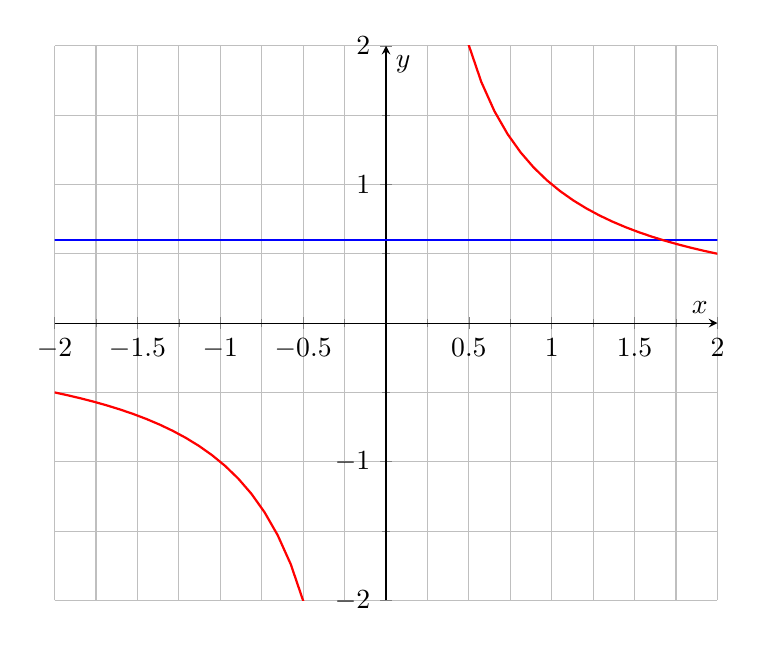
\begin{tikzpicture}
                \begin{axis}[grid=both,ymin=-2,ymax=2,xmax=2,xmin=-2,
                             minor tick num=1,axis lines = middle,xlabel=$x$,ylabel=$y$]
                    \addplot[color=blue, thick]{0.6};
                    \addplot[color=red, thick, domain=-2:-0.1]{1/x};
                    \addplot[color=red, thick, domain=0.1:2]{1/x};
                \end{axis}
            \end{tikzpicture}
        \end{center}
        Berdasarkan letak perpotongan pada grafik, diperoleh informasi bahwa fungsi memiliki satu akar $x$. \\
        
        Grafik diperbesar pada akar $x$:
        \begin{center}
            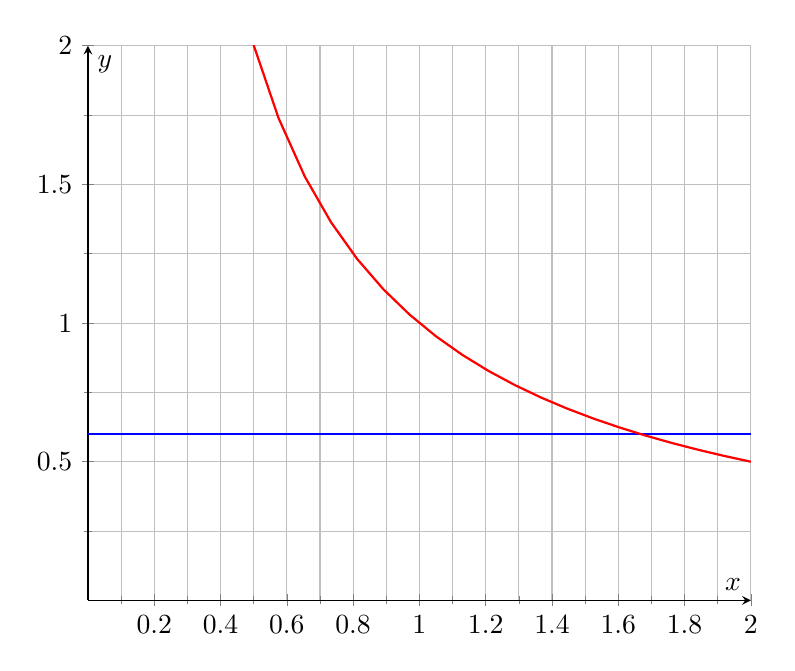
\begin{tikzpicture}
                \begin{axis}[grid=both,ymin=0,ymax=2,xmax=2,xmin=0,
                             minor tick num=1,axis lines = middle,xlabel=$x$,ylabel=$y$]
                    \addplot[color=blue, thick]{0.6};
                    \addplot[color=red, thick, domain=-2:-0.1]{1/x};
                    \addplot[color=red, thick, domain=0.1:2]{1/x};
                \end{axis}
            \end{tikzpicture}
        \end{center}
        Dengan demikian, dapat dipastikan bahwa akar $x$ berada di sekitar $(\num{1,6}; \num{1,7})$. \\

        \item $\num{9,36} - \num{21,963}x + \num{16,2965}x^2 - \num{3,70377}x^3$ \\
        \penyelesaian Hasil plotting dari persamaan tersebut diperoleh sebagai berikut.
        \begin{center}
            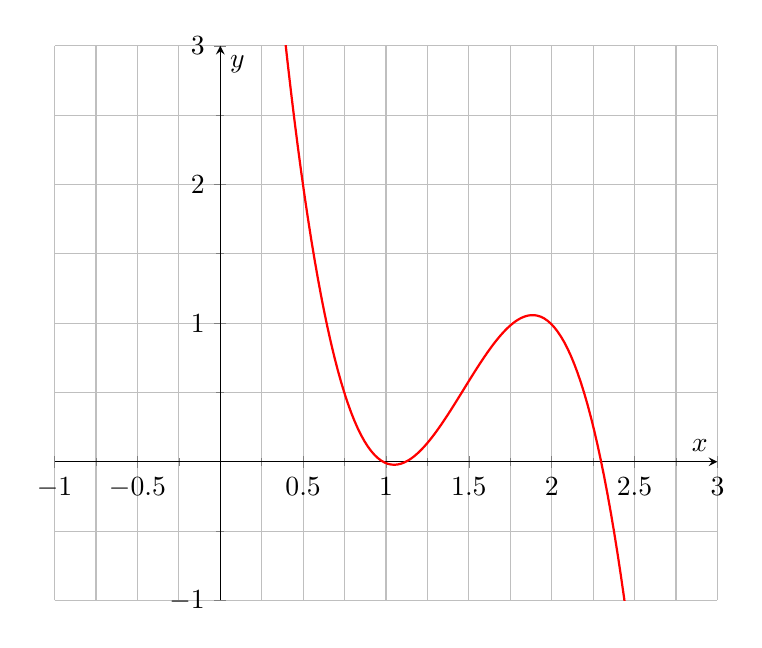
\begin{tikzpicture}
                \begin{axis}[grid=both,ymin=-1,ymax=3,xmax=3,xmin=-1,
                             minor tick num=1,axis lines = middle,xlabel=$x$,ylabel=$y$]
                    \addplot[color=red, thick, domain=-1:3, samples=200]{9.36 - 21.963*x + 16.2965*x^2 - 3.70377*x^3};
                \end{axis}
            \end{tikzpicture}
        \end{center}
        Berdasarkan letak perpotongan pada grafik, diperoleh informasi bahwa fungsi memiliki tiga akar, yakni $x_1$, $x_2$, dan $x_3$. 
        Dimana $x_1$ terletak di antara $(0, 1)$, $x_2$ terletak di antara $(1, 2)$, dan $x_3$ terletak di antara $(2, 3)$. \\
    \end{enumerate}

    \item Sekarang lengkapi jawaban no. 1 di atas dengan metode Tabulasi. \\
    \penyelesaian 
    \begin{enumerate}
        \item $e^x - x - 2 = 0$ \\
        Tabulasi akar $x_1$: \\
        \begin{tabular}{|c|c|}
            \hline
            $x$   & $f(x)$ \\
            \hline
            \num{-2,0} & \num{0,1353} \\
            \textcolor{red}{\num{-1,9}} & \textcolor{red}{\num{0,0496}} \\
            \textcolor{red}{\num{-1,8}} & \textcolor{red}{\num{-0,0347}} \\
            \num{-1,7} & \num{-0,1173} \\
            \num{-1,6} & \num{-0,1981} \\
            \num{-1,5} & \num{-0,2769} \\
            \num{-1,4} & \num{-0,3534} \\
            \num{-1,3} & \num{-0,4275} \\
            \num{-1,2} & \num{-0,4988} \\
            \num{-1,1} & \num{-0,5671} \\
            \num{-1,0} & \num{-0,6321} \\
            \hline
            \end{tabular}\quad
            \begin{tabular}{|c|c|}
            \hline
            $x$   & $f(x)$ \\
            \hline
            \num{-1,90} & \num{0,0496} \\
            \num{-1,89} & \num{0,0411} \\
            \num{-1,88} & \num{0,0326} \\
            \num{-1,87} & \num{0,0241} \\
            \num{-1,86} & \num{0,0157} \\
            \textcolor{red}{\num{-1,85}} & \textcolor{red}{\num{0,0072}} \\
            \textcolor{red}{\num{-1,84}} & \textcolor{red}{\num{-0,0012}} \\
            \num{-1,83} & \num{-0,0096} \\
            \num{-1,82} & \num{-0,0180} \\
            \num{-1,81} & \num{-0,0263} \\
            \num{-1,80} & \num{-0,0347} \\
            \hline
            \end{tabular}\quad
            \begin{tabular}{|c|c|}
            \hline
            $x$   & $f(x)$ \\
            \hline
            \num{-1,850} & \num{0,0072} \\
            \num{-1,849} & \num{0,0064} \\
            \num{-1,848} & \num{0,0056} \\
            \num{-1,847} & \num{0,0047} \\
            \num{-1,846} & \num{0,0039} \\
            \num{-1,845} & \num{0,0030} \\
            \num{-1,844} & \num{0,0022} \\
            \num{-1,843} & \num{0,0013} \\
            \textcolor{red}{\num{-1,842}} & \textcolor{red}{\num{0,0005}} \\
            \textcolor{red}{\num{-1,841}} & \textcolor{red}{\num{-0,0003}} \\
            \num{-1,840} & \num{-0,0012} \\
            \hline
            \end{tabular}\quad
            \begin{tabular}{|c|c|}
            \hline
            $x$   & $f(x)$ \\
            \hline
            \num{-1,8420} & \num{0,0005} \\
            \num{-1,8419} & \num{0,0004} \\
            \num{-1,8418} & \num{0,0003} \\
            \num{-1,8417} & \num{0,0002} \\
            \num{-1,8416} & \num{0,0002} \\
            \textcolor{red}{\num{-1,8415}} & \textcolor{red}{\num{0,0001}} \\
            \textcolor{red}{\num{-1,8414}} & \textcolor{red}{\num{-0,0000}} \\
            \num{-1,8413} & \num{-0,0001} \\
            \num{-1,8412} & \num{-0,0002} \\
            \num{-1,8411} & \num{-0,0003} \\
            \num{-1,8410} & \num{-0,0003} \\
            \hline
            \end{tabular}\quad \\
    
        Tabulasi akar $x_2$: \\ 
        \begin{tabular}{|c|c|}
            \hline
            $x$   & $f(x)$ \\
            \hline
            \num{1,0} & \num{-0,2817} \\
            \textcolor{red}{\num{1,1}} & \textcolor{red}{\num{-0,0958}} \\
            \textcolor{red}{\num{1,2}} & \textcolor{red}{\num{0,1201}} \\
            \num{1,3} & \num{0,3693} \\
            \num{1,4} & \num{0,6552} \\
            \num{1,5} & \num{0,9817} \\
            \num{1,6} & \num{1,3530} \\
            \num{1,7} & \num{1,7739} \\
            \num{1,8} & \num{2,2496} \\
            \num{1,9} & \num{2,7859} \\
            \num{2,0} & \num{3,3891} \\
            \hline
            \end{tabular}\quad
            \begin{tabular}{|c|c|}
            \hline
            $x$   & $f(x)$ \\
            \hline
            \num{1,10} & \num{-0,0958} \\
            \num{1,11} & \num{-0,0756} \\
            \num{1,12} & \num{-0,0551} \\
            \num{1,13} & \num{-0,0343} \\
            \textcolor{red}{\num{1,14}} & \textcolor{red}{\num{-0,0132}} \\
            \textcolor{red}{\num{1,15}} & \textcolor{red}{\num{0,0082}} \\
            \num{1,16} & \num{0,0299} \\
            \num{1,17} & \num{0,0520} \\
            \num{1,18} & \num{0,0744} \\
            \num{1,19} & \num{0,0971} \\
            \num{1,20} & \num{0,1201} \\
            \hline
            \end{tabular}\quad
            \begin{tabular}{|c|c|}
            \hline
            $x$   & $f(x)$ \\
            \hline
            \num{1,140} & \num{-0,0132} \\
            \num{1,141} & \num{-0,0111} \\
            \num{1,142} & \num{-0,0090} \\
            \num{1,143} & \num{-0,0068} \\
            \num{1,144} & \num{-0,0047} \\
            \num{1,145} & \num{-0,0026} \\
            \textcolor{red}{\num{1,146}} & \textcolor{red}{\num{-0,0004}} \\
            \textcolor{red}{\num{1,147}} & \textcolor{red}{\num{0,0017}} \\
            \num{1,148} & \num{0,0039} \\
            \num{1,149} & \num{0,0060} \\
            \num{1,150} & \num{0,0082} \\
            \hline
            \end{tabular}\quad
            \begin{tabular}{|c|c|}
            \hline
            $x$   & $f(x)$ \\
            \hline
            \num{1,1460} & \num{-0,0004} \\
            \textcolor{red}{\num{1,1461}} & \textcolor{red}{\num{-0,0002}} \\
            \textcolor{red}{\num{1,1462}} & \textcolor{red}{\num{0,0000}} \\
            \num{1,1463} & \num{0,0002} \\
            \num{1,1464} & \num{0,0004} \\
            \num{1,1465} & \num{0,0007} \\
            \num{1,1466} & \num{0,0009} \\
            \num{1,1467} & \num{0,0011} \\
            \num{1,1468} & \num{0,0013} \\
            \num{1,1469} & \num{0,0015} \\
            \num{1,1470} & \num{0,0017} \\
            \hline
            \end{tabular}\quad \\
    
        Dengan demikian, akar-akar dari $e^x - x - 2 = 0$, antara lain $x_1 \approx \num{-1,8414}$ dan $x_2 \approx \num{1,1462}$.\\
    
        \item $10^x = 100 - 2x$. \\
        Tabulasi akar $x$: \\
        \begin{tabular}{|c|c|}
            \hline
            $x$   & $f(x)$ \\
            \hline
            \num{1,90} & \num{-16,7672} \\
            \num{1,91} & \num{-14,8969} \\
            \num{1,92} & \num{-12,9836} \\
            \num{1,93} & \num{-11,0262} \\
            \num{1,94} & \num{-9,0236} \\
            \num{1,95} & \num{-6,9749} \\
            \num{1,96} & \num{-4,8789} \\
            \num{1,97} & \num{-2,7346} \\
            \textcolor{red}{\num{1,98}} & \textcolor{red}{\num{-0,5407}} \\
            \textcolor{red}{\num{1,99}} & \textcolor{red}{\num{1,7037}} \\
            \num{2,00} & \num{4,0000} \\
            \hline
            \end{tabular}\quad
            \begin{tabular}{|c|c|}
            \hline
            $x$   & $f(x)$ \\
            \hline
            \num{1,980} & \num{-0,5407} \\
            \num{1,981} & \num{-0,3186} \\
            \textcolor{red}{\num{1,982}} & \textcolor{red}{\num{-0,0959}} \\
            \textcolor{red}{\num{1,983}} & \textcolor{red}{\num{0,1272}} \\
            \num{1,984} & \num{0,3509} \\
            \num{1,985} & \num{0,5751} \\
            \num{1,986} & \num{0,7998} \\
            \num{1,987} & \num{1,0250} \\
            \num{1,988} & \num{1,2507} \\
            \num{1,989} & \num{1,4770} \\
            \num{1,990} & \num{1,7037} \\
            \hline
            \end{tabular}\quad
            \begin{tabular}{|c|c|}
            \hline
            $x$   & $f(x)$ \\
            \hline
            \num{1,9820} & \num{-0,0959} \\
            \num{1,9821} & \num{-0,0736} \\
            \num{1,9822} & \num{-0,0513} \\
            \num{1,9823} & \num{-0,0290} \\
            \textcolor{red}{\num{1,9824}} & \textcolor{red}{\num{-0,0067}} \\
            \textcolor{red}{\num{1,9825}} & \textcolor{red}{\num{0,0156}} \\
            \num{1,9826} & \num{0,0379} \\
            \num{1,9827} & \num{0,0602} \\
            \num{1,9828} & \num{0,0826} \\
            \num{1,9829} & \num{0,1049} \\
            \num{1,9830} & \num{0,1272} \\
            \hline
            \end{tabular}\quad
            \begin{tabular}{|c|c|}
            \hline
            $x$   & $f(x)$ \\
            \hline
            \num{1,98240} & \num{-0,0067} \\
            \num{1,98241} & \num{-0,0045} \\
            \num{1,98242} & \num{-0,0023} \\
            \textcolor{red}{\num{1,98243}} & \textcolor{red}{\num{-0,0000}} \\
            \textcolor{red}{\num{1,98244}} & \textcolor{red}{\num{0,0022}} \\
            \num{1,98245} & \num{0,0044} \\
            \num{1,98246} & \num{0,0067} \\
            \num{1,98247} & \num{0,0089} \\
            \num{1,98248} & \num{0,0111} \\
            \num{1,98249} & \num{0,0134} \\
            \num{1,98250} & \num{0,0156} \\
            \hline
            \end{tabular}\quad \\
            
        Dengan demikian, akar dari $10^x = 100 - 2x$ adalah $x \approx \num{1,98243}$.
    
        \item $\num{-0,874}x^2 + \num{1,75}x + \num{2,627}$ \\
        Tabulasi akar $x_1$:\\
        \begin{tabular}{|c|c|}
            \hline
            $x$   & $f(x)$ \\
            \hline
            \num{-1,10} & \num{-0,3555} \\
            \num{-1,09} & \num{-0,3189} \\
            \num{-1,08} & \num{-0,2824} \\
            \num{-1,07} & \num{-0,2461} \\
            \num{-1,06} & \num{-0,2100} \\
            \num{-1,05} & \num{-0,1741} \\
            \num{-1,04} & \num{-0,1383} \\
            \num{-1,03} & \num{-0,1027} \\
            \num{-1,02} & \num{-0,0673} \\
            \textcolor{red}{\num{-1,01}} & \textcolor{red}{\num{-0,0321}} \\
            \textcolor{red}{\num{-1,00}} & \textcolor{red}{\num{0,0030}} \\
            \hline
            \end{tabular}\quad
            \begin{tabular}{|c|c|}
            \hline
            $x$   & $f(x)$ \\
            \hline
            \num{-1,010} & \num{-0,0321} \\
            \num{-1,009} & \num{-0,0286} \\
            \num{-1,008} & \num{-0,0250} \\
            \num{-1,007} & \num{-0,0215} \\
            \num{-1,006} & \num{-0,0180} \\
            \num{-1,005} & \num{-0,0145} \\
            \num{-1,004} & \num{-0,0110} \\
            \num{-1,003} & \num{-0,0075} \\
            \num{-1,002} & \num{-0,0040} \\
            \textcolor{red}{\num{-1,001}} & \textcolor{red}{\num{-0,0005}} \\
            \textcolor{red}{\num{-1,000}} & \textcolor{red}{\num{0,0030}} \\
            \hline
            \end{tabular}\quad
            \begin{tabular}{|c|c|}
            \hline
            $x$   & $f(x)$ \\
            \hline
            \num{-1,0010} & \num{-0,0005} \\
            \textcolor{red}{\num{-1,0009}} & \textcolor{red}{\num{-0,0001}} \\
            \textcolor{red}{\num{-1,0008}} & \textcolor{red}{\num{0,0002}} \\
            \num{-1,0007} & \num{0,0006} \\
            \num{-1,0006} & \num{0,0009} \\
            \num{-1,0005} & \num{0,0013} \\
            \num{-1,0004} & \num{0,0016} \\
            \num{-1,0003} & \num{0,0020} \\
            \num{-1,0002} & \num{0,0023} \\
            \num{-1,0001} & \num{0,0027} \\
            \num{-1,0000} & \num{0,0030} \\
            \hline
            \end{tabular}\quad
            \begin{tabular}{|c|c|}
            \hline
            $x$   & $f(x)$ \\
            \hline
            \num{-1,00090} & \num{-0,0001} \\
            \num{-1,00089} & \num{-0,0001} \\
            \num{-1,00088} & \num{-0,0001} \\
            \num{-1,00087} & \num{-0,0000} \\
            \textcolor{red}{\num{-1,00086}} & \textcolor{red}{\num{-0,0000}} \\
            \textcolor{red}{\num{-1,00085}} & \textcolor{red}{\num{0,0000}} \\
            \num{-1,00084} & \num{0,0001} \\
            \num{-1,00083} & \num{0,0001} \\
            \num{-1,00082} & \num{0,0001} \\
            \num{-1,00081} & \num{0,0002} \\
            \num{-1,00080} & \num{0,0002} \\
            \hline
            \end{tabular}\quad \\            
            
            Tabulasi akar $x_2$: \\
            \begin{tabular}{|c|c|}
                \hline
                $x$   & $f(x)$ \\
                \hline
                \textcolor{red}{\num{3,00}} & \textcolor{red}{\num{0,0110}} \\
                \textcolor{red}{\num{3,01}} & \textcolor{red}{\num{-0,0240}} \\
                \num{3,02} & \num{-0,0592} \\
                \num{3,03} & \num{-0,0946} \\
                \num{3,04} & \num{-0,1302} \\
                \num{3,05} & \num{-0,1659} \\
                \num{3,06} & \num{-0,2018} \\
                \num{3,07} & \num{-0,2379} \\
                \num{3,08} & \num{-0,2741} \\
                \num{3,09} & \num{-0,3105} \\
                \num{3,10} & \num{-0,3471} \\
                \hline
                \end{tabular}\quad
                \begin{tabular}{|c|c|}
                \hline
                $x$   & $f(x)$ \\
                \hline
                \num{3,000} & \num{0,0110} \\
                \num{3,001} & \num{0,0075} \\
                \num{3,002} & \num{0,0040} \\
                \textcolor{red}{\num{3,003}} & \textcolor{red}{\num{0,0005}} \\
                \textcolor{red}{\num{3,004}} & \textcolor{red}{\num{-0,0030}} \\
                \num{3,005} & \num{-0,0065} \\
                \num{3,006} & \num{-0,0100} \\
                \num{3,007} & \num{-0,0135} \\
                \num{3,008} & \num{-0,0170} \\
                \num{3,009} & \num{-0,0205} \\
                \num{3,010} & \num{-0,0240} \\
                \hline
                \end{tabular}\quad
                \begin{tabular}{|c|c|}
                \hline
                $x$   & $f(x)$ \\
                \hline
                \num{3,0030} & \num{0,0005} \\
                \textcolor{red}{\num{3,0031}} & \textcolor{red}{\num{0,0002}} \\
                \textcolor{red}{\num{3,0032}} & \textcolor{red}{\num{-0,0002}} \\
                \num{3,0033} & \num{-0,0005} \\
                \num{3,0034} & \num{-0,0009} \\
                \num{3,0035} & \num{-0,0012} \\
                \num{3,0036} & \num{-0,0016} \\
                \num{3,0037} & \num{-0,0019} \\
                \num{3,0038} & \num{-0,0023} \\
                \num{3,0039} & \num{-0,0026} \\
                \num{3,0040} & \num{-0,0030} \\
                \hline
                \end{tabular}\quad
                \begin{tabular}{|c|c|}
                \hline
                $x$   & $f(x)$ \\
                \hline
                \num{3,00310} & \num{0,0002} \\
                \num{3,00311} & \num{0,0001} \\
                \num{3,00312} & \num{0,0001} \\
                \num{3,00313} & \num{0,0001} \\
                \textcolor{red}{\num{3,00314}} & \textcolor{red}{\num{0,0000}} \\
                \textcolor{red}{\num{3,00315}} & \textcolor{red}{\num{-0,0000}} \\
                \num{3,00316} & \num{-0,0000} \\
                \num{3,00317} & \num{-0,0001} \\
                \num{3,00318} & \num{-0,0001} \\
                \num{3,00319} & \num{-0,0002} \\
                \num{3,00320} & \num{-0,0002} \\
                \hline
                \end{tabular}\quad \\                   
    
            Dengan demikian, akar-akarnya adalah $x_1 \approx \num{-1,00086}$ dan $x_2 \approx \num{3,00314}$.
    
        \item $\num{-2,1} + \num{6,21}x - \num{3,9}x^2 + \num{0,667}x^3$ \\
        Tabulasi akar $x_1$: \\
        \begin{tabular}{|c|c|}
            \hline
            $x$   & $f(x)$ \\
            \hline
            \num{0,40} & \num{-0,1973} \\
            \num{0,41} & \num{-0,1635} \\
            \num{0,42} & \num{-0,1303} \\
            \num{0,43} & \num{-0,0978} \\
            \num{0,44} & \num{-0,0658} \\
            \num{0,45} & \num{-0,0345} \\
            \textcolor{red}{\num{0,46}} & \textcolor{red}{\num{-0,0037}} \\
            \textcolor{red}{\num{0,47}} & \textcolor{red}{\num{0,0264}} \\
            \num{0,48} & \num{0,0560} \\
            \num{0,49} & \num{0,0850} \\
            \num{0,50} & \num{0,1134} \\
            \hline
            \end{tabular}\quad
            \begin{tabular}{|c|c|}
            \hline
            $x$   & $f(x)$ \\
            \hline
            \num{0,460} & \num{-0,0037} \\
            \textcolor{red}{\num{0,461}} & \textcolor{red}{\num{-0,0007}} \\
            \textcolor{red}{\num{0,462}} & \textcolor{red}{\num{0,0024}} \\
            \num{0,463} & \num{0,0054} \\
            \num{0,464} & \num{0,0084} \\
            \num{0,465} & \num{0,0114} \\
            \num{0,466} & \num{0,0144} \\
            \num{0,467} & \num{0,0175} \\
            \num{0,468} & \num{0,0205} \\
            \num{0,469} & \num{0,0235} \\
            \num{0,470} & \num{0,0264} \\
            \hline
            \end{tabular}\quad
            \begin{tabular}{|c|c|}
            \hline
            $x$   & $f(x)$ \\
            \hline
            \num{0,4610} & \num{-0,0007} \\
            \num{0,4611} & \num{-0,0004} \\
            \textcolor{red}{\num{0,4612}} & \textcolor{red}{\num{-0,0001}} \\
            \textcolor{red}{\num{0,4613}} & \textcolor{red}{\num{0,0002}} \\
            \num{0,4614} & \num{0,0005} \\
            \num{0,4615} & \num{0,0008} \\
            \num{0,4616} & \num{0,0011} \\
            \num{0,4617} & \num{0,0015} \\
            \num{0,4618} & \num{0,0018} \\
            \num{0,4619} & \num{0,0021} \\
            \num{0,4620} & \num{0,0024} \\
            \hline
            \end{tabular}\quad
            \begin{tabular}{|c|c|}
            \hline
            $x$   & $f(x)$ \\
            \hline
            \num{0,46120} & \num{-0,0001} \\
            \num{0,46121} & \num{-0,0000} \\
            \textcolor{red}{\num{0,46122}} & \textcolor{red}{\num{-0,0000}} \\
            \textcolor{red}{\num{0,46123}} & \textcolor{red}{\num{0,0000}} \\
            \num{0,46124} & \num{0,0001} \\
            \num{0,46125} & \num{0,0001} \\
            \num{0,46126} & \num{0,0001} \\
            \num{0,46127} & \num{0,0001} \\
            \num{0,46128} & \num{0,0002} \\
            \num{0,46129} & \num{0,0002} \\
            \num{0,46130} & \num{0,0002} \\
            \hline
            \end{tabular}\quad \\
    
        Tabulasi akar $x_2$: \\
        \begin{tabular}{|c|c|}
            \hline
            $x$   & $f(x)$ \\
            \hline
            \num{2,00} & \num{0,0560} \\
            \num{2,01} & \num{0,0422} \\
            \num{2,02} & \num{0,0283} \\
            \num{2,03} & \num{0,0145} \\
            \textcolor{red}{\num{2,04}} & \textcolor{red}{\num{0,0008}} \\
            \textcolor{red}{\num{2,05}} & \textcolor{red}{\num{-0,0130}} \\
            \num{2,06} & \num{-0,0266} \\
            \num{2,07} & \num{-0,0403} \\
            \num{2,08} & \num{-0,0539} \\
            \num{2,09} & \num{-0,0674} \\
            \num{2,10} & \num{-0,0809} \\
            \hline
            \end{tabular}\quad
            \begin{tabular}{|c|c|}
            \hline
            $x$   & $f(x)$ \\
            \hline
            \textcolor{red}{\num{2,040}} & \textcolor{red}{\num{0,0008}} \\
            \textcolor{red}{\num{2,041}} & \textcolor{red}{\num{-0,0006}} \\
            \num{2,042} & \num{-0,0020} \\
            \num{2,043} & \num{-0,0034} \\
            \num{2,044} & \num{-0,0047} \\
            \num{2,045} & \num{-0,0061} \\
            \num{2,046} & \num{-0,0075} \\
            \num{2,047} & \num{-0,0088} \\
            \num{2,048} & \num{-0,0102} \\
            \num{2,049} & \num{-0,0116} \\
            \num{2,050} & \num{-0,0130} \\
            \hline
            \end{tabular}\quad
            \begin{tabular}{|c|c|}
            \hline
            $x$   & $f(x)$ \\
            \hline
            \num{2,0400} & \num{0,0008} \\
            \num{2,0401} & \num{0,0006} \\
            \num{2,0402} & \num{0,0005} \\
            \num{2,0403} & \num{0,0004} \\
            \num{2,0404} & \num{0,0002} \\
            \textcolor{red}{\num{2,0405}} & \textcolor{red}{\num{0,0001}} \\
            \textcolor{red}{\num{2,0406}} & \textcolor{red}{\num{-0,0001}} \\
            \num{2,0407} & \num{-0,0002} \\
            \num{2,0408} & \num{-0,0003} \\
            \num{2,0409} & \num{-0,0005} \\
            \num{2,0410} & \num{-0,0006} \\
            \hline
            \end{tabular}\quad
            \begin{tabular}{|c|c|}
            \hline
            $x$   & $f(x)$ \\
            \hline
            \num{2,04050} & \num{0,0001} \\
            \num{2,04051} & \num{0,0001} \\
            \num{2,04052} & \num{0,0001} \\
            \num{2,04053} & \num{0,0000} \\
            \num{2,04054} & \num{0,0000} \\
            \textcolor{red}{\num{2,04055}} & \textcolor{red}{\num{0,0000}} \\
            \textcolor{red}{\num{2,04056}} & \textcolor{red}{\num{-0,0000}} \\
            \num{2,04057} & \num{-0,0000} \\
            \num{2,04058} & \num{-0,0000} \\
            \num{2,04059} & \num{-0,0000} \\
            \num{2,04060} & \num{-0,0001} \\
            \hline
            \end{tabular}\quad \\         
            
        Dengan demikian, akar-akarnya adalah $x_1 \approx \num{0,46122}$ dan $x_2 \approx \num{2,04056}$.
    
        \item $(1 - \num{0,6}x)/x$ \\
        Tabulasi akar $x$: \\
        \begin{tabular}{|c|c|}
            \hline
            $x$   & $f(x)$ \\
            \hline
            \num{1,60} & \num{0,0250} \\
            \num{1,61} & \num{0,0211} \\
            \num{1,62} & \num{0,0173} \\
            \num{1,63} & \num{0,0135} \\
            \num{1,64} & \num{0,0098} \\
            \num{1,65} & \num{0,0061} \\
            \textcolor{red}{\num{1,66}} & \textcolor{red}{\num{0,0024}} \\
            \textcolor{red}{\num{1,67}} & \textcolor{red}{\num{-0,0012}} \\
            \num{1,68} & \num{-0,0048} \\
            \num{1,69} & \num{-0,0083} \\
            \num{1,70} & \num{-0,0118} \\
            \hline
            \end{tabular}\quad
            \begin{tabular}{|c|c|}
            \hline
            $x$   & $f(x)$ \\
            \hline
            \num{1,660} & \num{0,0024} \\
            \num{1,661} & \num{0,0020} \\
            \num{1,662} & \num{0,0017} \\
            \num{1,663} & \num{0,0013} \\
            \num{1,664} & \num{0,0010} \\
            \num{1,665} & \num{0,0006} \\
            \textcolor{red}{\num{1,666}} & \textcolor{red}{\num{0,0002}} \\
            \textcolor{red}{\num{1,667}} & \textcolor{red}{\num{-0,0001}} \\
            \num{1,668} & \num{-0,0005} \\
            \num{1,669} & \num{-0,0008} \\
            \num{1,670} & \num{-0,0012} \\
            \hline
            \end{tabular}\quad
            \begin{tabular}{|c|c|}
            \hline
            $x$   & $f(x)$ \\
            \hline
            \num{1,6660} & \num{0,0002} \\
            \num{1,6661} & \num{0,0002} \\
            \num{1,6662} & \num{0,0002} \\
            \num{1,6663} & \num{0,0001} \\
            \num{1,6664} & \num{0,0001} \\
            \num{1,6665} & \num{0,0001} \\
            \textcolor{red}{\num{1,6666}} & \textcolor{red}{\num{0,0000}} \\
            \textcolor{red}{\num{1,6667}} & \textcolor{red}{\num{-0,0000}} \\
            \num{1,6668} & \num{-0,0000} \\
            \num{1,6669} & \num{-0,0001} \\
            \num{1,6670} & \num{-0,0001} \\
            \hline
            \end{tabular}\quad
            \begin{tabular}{|c|c|}
            \hline
            $x$   & $f(x)$ \\
            \hline
            \num{1,66660} & \num{0,0000} \\
            \num{1,66661} & \num{0,0000} \\
            \num{1,66662} & \num{0,0000} \\
            \num{1,66663} & \num{0,0000} \\
            \num{1,66664} & \num{0,0000} \\
            \num{1,66665} & \num{0,0000} \\
            \textcolor{red}{\num{1,66666}} & \textcolor{red}{\num{0,0000}} \\
            \textcolor{red}{\num{1,66667}} & \textcolor{red}{\num{-0,0000}} \\
            \num{1,66668} & \num{-0,0000} \\
            \num{1,66669} & \num{-0,0000} \\
            \num{1,66670} & \num{-0,0000} \\
            \hline
            \end{tabular}\quad \\ 
    
        Dengan demikian, akar dari $(1 - \num{0,6}x) / x$ adalah $x \approx \num{1,66667}$.
    
        \item $\num{9,36} - \num{21,963}x + \num{16,2965}x^2 - \num{3,70377}x^3$ \\
        Tabulasi akar $x_1$: \\
        \begin{tabular}{|c|c|}
            \hline
            $x$   & $f(x)$ \\
            \hline
            \num{0,0} & \num{9,3600} \\
            \num{0,1} & \num{7,3230} \\
            \num{0,2} & \num{5,5896} \\
            \num{0,3} & \num{4,1378} \\
            \num{0,4} & \num{2,9452} \\
            \num{0,5} & \num{1,9897} \\
            \num{0,6} & \num{1,2489} \\
            \num{0,7} & \num{0,7008} \\
            \num{0,8} & \num{0,3230} \\
            \textcolor{red}{\num{0,9}} & \textcolor{red}{\num{0,0934}} \\
            \textcolor{red}{\num{1,0}} & \textcolor{red}{\num{-0,0103}} \\
            \hline
            \end{tabular}\quad
            \begin{tabular}{|c|c|}
            \hline
            $x$   & $f(x)$ \\
            \hline
            \num{0,90} & \num{0,0934} \\
            \num{0,91} & \num{0,0777} \\
            \num{0,92} & \num{0,0633} \\
            \num{0,93} & \num{0,0501} \\
            \num{0,94} & \num{0,0381} \\
            \num{0,95} & \num{0,0272} \\
            \num{0,96} & \num{0,0175} \\
            \num{0,97} & \num{0,0089} \\
            \textcolor{red}{\num{0,98}} & \textcolor{red}{\num{0,0015}} \\
            \textcolor{red}{\num{0,99}} & \textcolor{red}{\num{-0,0049}} \\
            \num{1,00} & \num{-0,0103} \\
            \hline
            \end{tabular}\quad
            \begin{tabular}{|c|c|}
            \hline
            $x$   & $f(x)$ \\
            \hline
            \num{0,980} & \num{0,0015} \\
            \num{0,981} & \num{0,0008} \\
            \textcolor{red}{\num{0,982}} & \textcolor{red}{\num{0,0001}} \\
            \textcolor{red}{\num{0,983}} & \textcolor{red}{\num{-0,0006}} \\
            \num{0,984} & \num{-0,0012} \\
            \num{0,985} & \num{-0,0019} \\
            \num{0,986} & \num{-0,0025} \\
            \num{0,987} & \num{-0,0031} \\
            \num{0,988} & \num{-0,0037} \\
            \num{0,989} & \num{-0,0043} \\
            \num{0,990} & \num{-0,0049} \\
            \hline
            \end{tabular}\quad
            \begin{tabular}{|c|c|}
            \hline
            $x$   & $f(x)$ \\
            \hline
            \num{0,9820} & \num{0,0001} \\
            \textcolor{red}{\num{0,9821}} & \textcolor{red}{\num{0,0000}} \\
            \textcolor{red}{\num{0,9822}} & \textcolor{red}{\num{-0,0000}} \\
            \num{0,9823} & \num{-0,0001} \\
            \num{0,9824} & \num{-0,0002} \\
            \num{0,9825} & \num{-0,0002} \\
            \num{0,9826} & \num{-0,0003} \\
            \num{0,9827} & \num{-0,0004} \\
            \num{0,9828} & \num{-0,0004} \\
            \num{0,9829} & \num{-0,0005} \\
            \num{0,9830} & \num{-0,0006} \\
            \hline
            \end{tabular}\quad \\
            
        Tabulasi akar $x_2$: \\
        \begin{tabular}{|c|c|}
            \hline
            $x$   & $f(x)$ \\
            \hline
            \num{1,0} & \num{-0,0103} \\
            \textcolor{red}{\num{1,1}} & \textcolor{red}{\num{-0,0103}} \\
            \textcolor{red}{\num{1,2}} & \textcolor{red}{\num{0,0712}} \\
            \num{1,3} & \num{0,2120} \\
            \num{1,4} & \num{0,3898} \\
            \num{1,5} & \num{0,5824} \\
            \num{1,6} & \num{0,7676} \\
            \num{1,7} & \num{0,9232} \\
            \num{1,8} & \num{1,0269} \\
            \num{1,9} & \num{1,0565} \\
            \num{2,0} & \num{0,9898} \\
            \hline
            \end{tabular}\quad
            \begin{tabular}{|c|c|}
            \hline
            $x$   & $f(x)$ \\
            \hline
            \num{1,10} & \num{-0,0103} \\
            \textcolor{red}{\num{1,11}} & \textcolor{red}{\num{-0,0054}} \\
            \textcolor{red}{\num{1,12}} & \textcolor{red}{\num{0,0002}} \\
            \num{1,13} & \num{0,0067} \\
            \num{1,14} & \num{0,0138} \\
            \num{1,15} & \num{0,0217} \\
            \num{1,16} & \num{0,0303} \\
            \num{1,17} & \num{0,0396} \\
            \num{1,18} & \num{0,0495} \\
            \num{1,19} & \num{0,0601} \\
            \num{1,20} & \num{0,0712} \\
            \hline
            \end{tabular}\quad
            \begin{tabular}{|c|c|}
            \hline
            $x$   & $f(x)$ \\
            \hline
            \num{1,110} & \num{-0,0054} \\
            \num{1,111} & \num{-0,0049} \\
            \num{1,112} & \num{-0,0043} \\
            \num{1,113} & \num{-0,0038} \\
            \num{1,114} & \num{-0,0032} \\
            \num{1,115} & \num{-0,0027} \\
            \num{1,116} & \num{-0,0021} \\
            \num{1,117} & \num{-0,0015} \\
            \num{1,118} & \num{-0,0010} \\
            \textcolor{red}{\num{1,119}} & \textcolor{red}{\num{-0,0004}} \\
            \textcolor{red}{\num{1,120}} & \textcolor{red}{\num{0,0002}} \\
            \hline
            \end{tabular}\quad
            \begin{tabular}{|c|c|}
            \hline
            $x$   & $f(x)$ \\
            \hline
            \num{1,1190} & \num{-0,0004} \\
            \num{1,1191} & \num{-0,0003} \\
            \num{1,1192} & \num{-0,0002} \\
            \num{1,1193} & \num{-0,0002} \\
            \num{1,1194} & \num{-0,0001} \\
            \num{1,1195} & \num{-0,0001} \\
            \textcolor{red}{\num{1,1196}} & \textcolor{red}{\num{-0,0000}} \\
            \textcolor{red}{\num{1,1197}} & \textcolor{red}{\num{0,0001}} \\
            \num{1,1198} & \num{0,0001} \\
            \num{1,1199} & \num{0,0002} \\
            \num{1,1200} & \num{0,0002} \\
            \hline
            \end{tabular}\quad \\

        Tabulasi akar $x_3$: \\
        \begin{tabular}{|c|c|}
            \hline
            $x$   & $f(x)$ \\
            \hline
            \num{2,0} & \num{0,9898} \\
            \num{2,1} & \num{0,8047} \\
            \textcolor{red}{\num{2,2}} & \textcolor{red}{\num{0,4787}} \\
            \textcolor{red}{\num{2,3}} & \textcolor{red}{\num{-0,0102}} \\
            \num{2,4} & \num{-0,6843} \\
            \num{2,5} & \num{-1,5658} \\
            \num{2,6} & \num{-2,6769} \\
            \num{2,7} & \num{-4,0399} \\
            \num{2,8} & \num{-5,6770} \\
            \num{2,9} & \num{-7,6104} \\
            \num{3,0} & \num{-9,8623} \\
            \hline
            \end{tabular}\quad
            \begin{tabular}{|c|c|}
            \hline
            $x$   & $f(x)$ \\
            \hline
            \num{2,20} & \num{0,4787} \\
            \num{2,21} & \num{0,4375} \\
            \num{2,22} & \num{0,3947} \\
            \num{2,23} & \num{0,3502} \\
            \num{2,24} & \num{0,3040} \\
            \num{2,25} & \num{0,2560} \\
            \num{2,26} & \num{0,2064} \\
            \num{2,27} & \num{0,1549} \\
            \num{2,28} & \num{0,1017} \\
            \textcolor{red}{\num{2,29}} & \textcolor{red}{\num{0,0467}} \\
            \textcolor{red}{\num{2,30}} & \textcolor{red}{\num{-0,0102}} \\
            \hline
            \end{tabular}\quad
            \begin{tabular}{|c|c|}
            \hline
            $x$   & $f(x)$ \\
            \hline
            \num{2,290} & \num{0,0467} \\
            \num{2,291} & \num{0,0411} \\
            \num{2,292} & \num{0,0354} \\
            \num{2,293} & \num{0,0298} \\
            \num{2,294} & \num{0,0242} \\
            \num{2,295} & \num{0,0185} \\
            \num{2,296} & \num{0,0128} \\
            \num{2,297} & \num{0,0071} \\
            \textcolor{red}{\num{2,298}} & \textcolor{red}{\num{0,0013}} \\
            \textcolor{red}{\num{2,299}} & \textcolor{red}{\num{-0,0044}} \\
            \num{2,300} & \num{-0,0102} \\
            \hline
            \end{tabular}\quad
            \begin{tabular}{|c|c|}
            \hline
            $x$   & $f(x)$ \\
            \hline
            \num{2,2980} & \num{0,0013} \\
            \num{2,2981} & \num{0,0008} \\
            \textcolor{red}{\num{2,2982}} & \textcolor{red}{\num{0,0002}} \\
            \textcolor{red}{\num{2,2983}} & \textcolor{red}{\num{-0,0004}} \\
            \num{2,2984} & \num{-0,0010} \\
            \num{2,2985} & \num{-0,0015} \\
            \num{2,2986} & \num{-0,0021} \\
            \num{2,2987} & \num{-0,0027} \\
            \num{2,2988} & \num{-0,0033} \\
            \num{2,2989} & \num{-0,0038} \\
            \num{2,2990} & \num{-0,0044} \\
            \hline
            \end{tabular}\quad \\
            Dengan demikian, akar-akar dari persamaan ini antara lain, $x_1 \approx \num{0,9822}$, $x_2 \approx \num{1,1196}$, dan $x_3 \approx \num{2,2982}$.
    \end{enumerate}

    \item Dengan metode Bolzano, dapatkan akar-akar persamaan:
    \begin{enumerate}
        \item $x^3 - 3x + 1 = 0$ ($x_0 = \num{1,5}$; s.d. 3 digit) \\
        \penyelesaian \\
        \begin{tabular}{|c|c|c|c|c|c|c|}
            \hline
            iterasi & $x_1$ & $x_2$ & $x_3$ & $f(x_1)$ & $f(x_2)$ & $f(x_3)$ \\
            \hline
            1 & \num{1,000} & \num{2,000} & \num{1,500} & \num{-1,000} & \num{3,000} & \num{-0,125}\\
            2 & \num{1,500} & \num{2,000} & \num{1,750} & \num{-0,125} & \num{3,000} & \num{1,109}\\
            3 & \num{1,500} & \num{1,750} & \num{1,625} & \num{-0,125} & \num{1,109} & \num{0,416}\\
            4 & \num{1,500} & \num{1,625} & \num{1,562} & \num{-0,125} & \num{0,416} & \num{0,127}\\
            5 & \num{1,500} & \num{1,562} & \num{1,531} & \num{-0,125} & \num{0,127} & \num{-0,003}\\
            6 & \num{1,531} & \num{1,562} & \num{1,547} & \num{-0,003} & \num{0,127} & \num{0,061}\\
            7 & \num{1,531} & \num{1,547} & \num{1,539} & \num{-0,003} & \num{0,061} & \num{0,028}\\
            8 & \num{1,531} & \num{1,539} & \num{1,535} & \num{-0,003} & \num{0,028} & \num{0,012}\\
            9 & \num{1,531} & \num{1,535} & \num{1,533} & \num{-0,003} & \num{0,012} & \num{0,005}\\
            10 & \num{1,531} & \num{1,533} & \num{1,532} & \num{-0,003} & \num{0,005} & \num{0,001}\\
            11 & \num{1,531} & \num{1,532} & \num{1,532} & \num{-0,003} & \num{0,001} & \num{-0,001}\\
            12 & \num{1,532} & \num{1,532} & \num{1,532} & \num{-0,001} & \num{0,001} & \num{-0,000}\\
            13 & \num{1,532} & \num{1,532} & \num{1,532} & \num{-0,000} & \num{0,001} & \num{0,000}\\
             \hline
            \end{tabular} \\
        Dengan demikian, akar dari persamaan $x^3 - 3x + 1 = 0$ hingga 3 digit dibelakang koma adalah $x \approx \num{1,532}$.
            
        \item $\cos{x} = 3x$ ($x_0 = \num{0,3}$; s.d. 5 digit) \\
        \penyelesaian \\
        \begin{tabular}{|c|c|c|c|c|c|c|}
            \hline
            iterasi & $x_1$ & $x_2$ & $x_3$ & $f(x_1)$ & $f(x_2)$ & $f(x_3)$ \\
            \hline
            1 & \num{0,20000} & \num{0,40000} & \num{0,30000} & \num{0,38007} & \num{-0,27894} & \num{0,05534}\\
            2 & \num{0,30000} & \num{0,40000} & \num{0,35000} & \num{0,05534} & \num{-0,27894} & \num{-0,11063}\\
            3 & \num{0,30000} & \num{0,35000} & \num{0,32500} & \num{0,05534} & \num{-0,11063} & \num{-0,02735}\\
            4 & \num{0,30000} & \num{0,32500} & \num{0,31250} & \num{0,05534} & \num{-0,02735} & \num{0,01407}\\
            5 & \num{0,31250} & \num{0,32500} & \num{0,31875} & \num{0,01407} & \num{-0,02735} & \num{-0,00662}\\
            6 & \num{0,31250} & \num{0,31875} & \num{0,31563} & \num{0,01407} & \num{-0,00662} & \num{0,00373}\\
            7 & \num{0,31563} & \num{0,31875} & \num{0,31719} & \num{0,00373} & \num{-0,00662} & \num{-0,00145}\\
            8 & \num{0,31563} & \num{0,31719} & \num{0,31641} & \num{0,00373} & \num{-0,00145} & \num{0,00114}\\
            9 & \num{0,31641} & \num{0,31719} & \num{0,31680} & \num{0,00114} & \num{-0,00145} & \num{-0,00015}\\
            10 & \num{0,31641} & \num{0,31680} & \num{0,31660} & \num{0,00114} & \num{-0,00015} & \num{0,00049}\\
            11 & \num{0,31660} & \num{0,31680} & \num{0,31670} & \num{0,00049} & \num{-0,00015} & \num{0,00017}\\
            12 & \num{0,31670} & \num{0,31680} & \num{0,31675} & \num{0,00017} & \num{-0,00015} & \num{0,00001}\\
            13 & \num{0,31675} & \num{0,31680} & \num{0,31677} & \num{0,00001} & \num{-0,00015} & \num{-0,00007}\\
            14 & \num{0,31675} & \num{0,31677} & \num{0,31676} & \num{0,00001} & \num{-0,00007} & \num{-0,00003}\\
            15 & \num{0,31675} & \num{0,31676} & \num{0,31675} & \num{0,00001} & \num{-0,00003} & \num{-0,00001}\\
            16 & \num{0,31675} & \num{0,31675} & \num{0,31675} & \num{0,00001} & \num{-0,00001} & \num{-0,00000}\\
             \hline
            \end{tabular} \\                     
        Dengan demikian, akar dari persamaan $\cos{x} = 3x$ hingga 5 digit di belakang koma adalah $x \approx \num{0,31675}$.

        \item $10^x = 100 - 2x$ ($x_0 = \num{2}$; s.d. 4 digit) \\
        \penyelesaian \\         
        \begin{tabular}{|c|c|c|c|c|c|c|}
            \hline
            iterasi & $x_1$ & $x_2$ & $x_3$ & $f(x_1)$ & $f(x_2)$ & $f(x_3)$ \\
            \hline
            1 & \num{1,5000} & \num{2,5000} & \num{2,0000} & \num{-65,3772} & \num{221,2278} & \num{4,0000}\\
            2 & \num{1,5000} & \num{2,0000} & \num{1,7500} & \num{-65,3772} & \num{4,0000} & \num{-40,2659}\\
            3 & \num{1,7500} & \num{2,0000} & \num{1,8750} & \num{-40,2659} & \num{4,0000} & \num{-21,2606}\\
            4 & \num{1,8750} & \num{2,0000} & \num{1,9375} & \num{-21,2606} & \num{4,0000} & \num{-9,5286}\\
            5 & \num{1,9375} & \num{2,0000} & \num{1,9688} & \num{-9,5286} & \num{4,0000} & \num{-3,0053}\\
            6 & \num{1,9688} & \num{2,0000} & \num{1,9844} & \num{-3,0053} & \num{4,0000} & \num{0,4349}\\
            7 & \num{1,9688} & \num{1,9844} & \num{1,9766} & \num{-3,0053} & \num{0,4349} & \num{-1,3005}\\
            8 & \num{1,9766} & \num{1,9844} & \num{1,9805} & \num{-1,3005} & \num{0,4349} & \num{-0,4367}\\
            9 & \num{1,9805} & \num{1,9844} & \num{1,9824} & \num{-0,4367} & \num{0,4349} & \num{-0,0019}\\
            10 & \num{1,9824} & \num{1,9844} & \num{1,9834} & \num{-0,0019} & \num{0,4349} & \num{0,2163}\\
            11 & \num{1,9824} & \num{1,9834} & \num{1,9829} & \num{-0,0019} & \num{0,2163} & \num{0,1072}\\
            12 & \num{1,9824} & \num{1,9829} & \num{1,9827} & \num{-0,0019} & \num{0,1072} & \num{0,0526}\\
            13 & \num{1,9824} & \num{1,9827} & \num{1,9825} & \num{-0,0019} & \num{0,0526} & \num{0,0254}\\
            14 & \num{1,9824} & \num{1,9825} & \num{1,9825} & \num{-0,0019} & \num{0,0254} & \num{0,0118}\\
            15 & \num{1,9824} & \num{1,9825} & \num{1,9825} & \num{-0,0019} & \num{0,0118} & \num{0,0050}\\
            16 & \num{1,9824} & \num{1,9825} & \num{1,9824} & \num{-0,0019} & \num{0,0050} & \num{0,0016}\\
            17 & \num{1,9824} & \num{1,9824} & \num{1,9824} & \num{-0,0019} & \num{0,0016} & \num{-0,0001}\\
            18 & \num{1,9824} & \num{1,9824} & \num{1,9824} & \num{-0,0001} & \num{0,0016} & \num{0,0007}\\
            19 & \num{1,9824} & \num{1,9824} & \num{1,9824} & \num{-0,0001} & \num{0,0007} & \num{0,0003}\\
            20 & \num{1,9824} & \num{1,9824} & \num{1,9824} & \num{-0,0001} & \num{0,0003} & \num{0,0001}\\
            21 & \num{1,9824} & \num{1,9824} & \num{1,9824} & \num{-0,0001} & \num{0,0001} & \num{-0,0000}\\
            22 & \num{1,9824} & \num{1,9824} & \num{1,9824} & \num{-0,0000} & \num{0,0001} & \num{0,0000}\\
            23 & \num{1,9824} & \num{1,9824} & \num{1,9824} & \num{-0,0000} & \num{0,0000} & \num{-0,0000}\\
            24 & \num{1,9824} & \num{1,9824} & \num{1,9824} & \num{-0,0000} & \num{0,0000} & \num{-0,0000}\\
             \hline
            \end{tabular} \\           
        Dengan demikian, akar persamaan dari $10^x = 100 - 2x$ hingga 4 digit di belakang koma adalah $x \approx \num{1,9824}$.

        \item $\ln{x} = 1 + 1/x^2$ ($x_0 = \num{3}$; s.d. 4 digit) \\
        \penyelesaian \\
        \begin{tabular}{|c|c|c|c|c|c|c|}
            \hline
            iterasi & $x_1$ & $x_2$ & $x_3$ & $f(x_1)$ & $f(x_2)$ & $f(x_3)$ \\
            \hline
            1 & \num{2,5000} & \num{3,5000} & \num{3,0000} & \num{-0,2437} & \num{0,1711} & \num{-0,0125}\\
            2 & \num{3,0000} & \num{3,5000} & \num{3,2500} & \num{-0,0125} & \num{0,1711} & \num{0,0840}\\
            3 & \num{3,0000} & \num{3,2500} & \num{3,1250} & \num{-0,0125} & \num{0,0840} & \num{0,0370}\\
            4 & \num{3,0000} & \num{3,1250} & \num{3,0625} & \num{-0,0125} & \num{0,0370} & \num{0,0126}\\
            5 & \num{3,0000} & \num{3,0625} & \num{3,0312} & \num{-0,0125} & \num{0,0126} & \num{0,0001}\\
            6 & \num{3,0000} & \num{3,0312} & \num{3,0156} & \num{-0,0125} & \num{0,0001} & \num{-0,0062}\\
            7 & \num{3,0156} & \num{3,0312} & \num{3,0234} & \num{-0,0062} & \num{0,0001} & \num{-0,0030}\\
            8 & \num{3,0234} & \num{3,0312} & \num{3,0273} & \num{-0,0030} & \num{0,0001} & \num{-0,0014}\\
            9 & \num{3,0273} & \num{3,0312} & \num{3,0293} & \num{-0,0014} & \num{0,0001} & \num{-0,0006}\\
            10 & \num{3,0293} & \num{3,0312} & \num{3,0303} & \num{-0,0006} & \num{0,0001} & \num{-0,0002}\\
            11 & \num{3,0303} & \num{3,0312} & \num{3,0308} & \num{-0,0002} & \num{0,0001} & \num{-0,0001}\\
            12 & \num{3,0308} & \num{3,0312} & \num{3,0310} & \num{-0,0001} & \num{0,0001} & \num{0,0000}\\
            13 & \num{3,0308} & \num{3,0310} & \num{3,0309} & \num{-0,0001} & \num{0,0000} & \num{-0,0000}\\
             \hline
            \end{tabular} \\      
        Dengan demikian, akar persamaan dari $\ln{x} = 1 + 1/x^2$ hingga 4 digit di belakang koma adalah $x \approx \num{3,0309}$.     

        \item $e^x - \ln{x} = 20$ ($x_0 = \num{3}$; s.d. 5 digit) \\ 
        \penyelesaian \\
        \begin{tabular}{|c|c|c|c|c|c|c|}
            \hline
            iterasi & $x_1$ & $x_2$ & $x_3$ & $f(x_1)$ & $f(x_2)$ & $f(x_3)$ \\
            \hline
            1 & \num{2,50000} & \num{3,50000} & \num{3,00000} & \num{-8,73380} & \num{11,86269} & \num{-1,01308}\\
            2 & \num{3,00000} & \num{3,50000} & \num{3,25000} & \num{-1,01308} & \num{11,86269} & \num{4,61168}\\
            3 & \num{3,00000} & \num{3,25000} & \num{3,12500} & \num{-1,01308} & \num{4,61168} & \num{1,62046}\\
            4 & \num{3,00000} & \num{3,12500} & \num{3,06250} & \num{-1,01308} & \num{1,62046} & \num{0,26171}\\
            5 & \num{3,00000} & \num{3,06250} & \num{3,03125} & \num{-1,01308} & \num{0,26171} & \num{-0,38585}\\
            6 & \num{3,03125} & \num{3,06250} & \num{3,04688} & \num{-0,38585} & \num{0,26171} & \num{-0,06465}\\
            7 & \num{3,04688} & \num{3,06250} & \num{3,05469} & \num{-0,06465} & \num{0,26171} & \num{0,09788}\\
            8 & \num{3,04688} & \num{3,05469} & \num{3,05078} & \num{-0,06465} & \num{0,09788} & \num{0,01645}\\
            9 & \num{3,04688} & \num{3,05078} & \num{3,04883} & \num{-0,06465} & \num{0,01645} & \num{-0,02414}\\
            10 & \num{3,04883} & \num{3,05078} & \num{3,04980} & \num{-0,02414} & \num{0,01645} & \num{-0,00386}\\
            11 & \num{3,04980} & \num{3,05078} & \num{3,05029} & \num{-0,00386} & \num{0,01645} & \num{0,00629}\\
            12 & \num{3,04980} & \num{3,05029} & \num{3,05005} & \num{-0,00386} & \num{0,00629} & \num{0,00122}\\
            13 & \num{3,04980} & \num{3,05005} & \num{3,04993} & \num{-0,00386} & \num{0,00122} & \num{-0,00132}\\
            14 & \num{3,04993} & \num{3,05005} & \num{3,04999} & \num{-0,00132} & \num{0,00122} & \num{-0,00005}\\
            15 & \num{3,04999} & \num{3,05005} & \num{3,05002} & \num{-0,00005} & \num{0,00122} & \num{0,00058}\\
            16 & \num{3,04999} & \num{3,05002} & \num{3,05000} & \num{-0,00005} & \num{0,00058} & \num{0,00027}\\
            17 & \num{3,04999} & \num{3,05000} & \num{3,05000} & \num{-0,00005} & \num{0,00027} & \num{0,00011}\\
            18 & \num{3,04999} & \num{3,05000} & \num{3,04999} & \num{-0,00005} & \num{0,00011} & \num{0,00003}\\
            19 & \num{3,04999} & \num{3,04999} & \num{3,04999} & \num{-0,00005} & \num{0,00003} & \num{-0,00001}\\
            20 & \num{3,04999} & \num{3,04999} & \num{3,04999} & \num{-0,00001} & \num{0,00003} & \num{0,00001}\\
            21 & \num{3,04999} & \num{3,04999} & \num{3,04999} & \num{-0,00001} & \num{0,00001} & \num{-0,00000}\\
            22 & \num{3,04999} & \num{3,04999} & \num{3,04999} & \num{-0,00000} & \num{0,00001} & \num{0,00000}\\
            23 & \num{3,04999} & \num{3,04999} & \num{3,04999} & \num{-0,00000} & \num{0,00000} & \num{0,00000}\\
            24 & \num{3,04999} & \num{3,04999} & \num{3,04999} & \num{-0,00000} & \num{0,00000} & \num{-0,00000}\\
             \hline
            \end{tabular} \\           
        Dengan demikian, akar persamaan dari $e^x - \ln{x} = 20$ hingga 5 digit di belakang koma adalah $x \approx \num{3,04999}$.  

        \item $10^x - 1$ ($x_0 = \num{0}$; s.d. 4 digit) \\ 
        \penyelesaian \\
        \begin{tabular}{|c|c|c|c|c|c|c|}
            \hline
            iterasi & $x_1$ & $x_2$ & $x_3$ & $f(x_1)$ & $f(x_2)$ & $f(x_3)$ \\
            \hline
            1 & \num{-0,5000} & \num{1,5000} & \num{0,5000} & \num{-0,6838} & \num{30,6228} & \num{2,1623}\\
            2 & \num{-0,5000} & \num{0,5000} & \num{0,0000} & \num{-0,6838} & \num{2,1623} & \num{0,0000}\\
             \hline
            \end{tabular} \\
        Dengan demikian, akar persamaan $10^x - 1$ hingga 4 digit di belakang koma adalah $x \approx \num{0,0000}$;
    \end{enumerate}

    \item Dengan metode Regula Falsi, dapatkan akar-akar persamaan:
    \begin{enumerate}
        \item $\sin x = 5x - 2$ ($x_0 = \num{0,4};$ s.d. 4 digit) \\
        \penyelesaian \\
        \begin{tabular}{|c|c|c|c|c|c|c|}
            \hline
            iterasi & $x_1$ & $x_2$ & $x_3$ & $f(x_1)$ & $f(x_2)$ & $f(x_3)$ \\
            \hline
            1 & \num{0,4000} & \num{1,0000} & \num{0,4917} & \num{0,3894} & \num{-2,1585} & \num{0,0136}\\
            2 & \num{0,4917} & \num{1,0000} & \num{0,4949} & \num{0,0136} & \num{-2,1585} & \num{0,0005}\\
            3 & \num{0,4949} & \num{1,0000} & \num{0,4950} & \num{0,0005} & \num{-2,1585} & \num{0,0000}\\
            4 & \num{0,4950} & \num{1,0000} & \num{0,4950} & \num{0,0000} & \num{-2,1585} & \num{0,0000}\\
             \hline
            \end{tabular}         \\   
        $\therefore x \approx \num{0,4950}$
    
        \item $e^x = 2x + 21$ ($x_0 = \num{3};$ s.d. 3 digit) \\
        \penyelesaian \\
        \begin{tabular}{|c|c|c|c|c|c|c|}
            \hline
            iterasi & $x_1$ & $x_2$ & $x_3$ & $f(x_1)$ & $f(x_2)$ & $f(x_3)$ \\
            \hline
            1 & \num{2,500} & \num{3,500} & \num{3,230} & \num{-13,818} & \num{5,115} & \num{-2,185}\\
            2 & \num{3,230} & \num{3,500} & \num{3,311} & \num{-2,185} & \num{5,115} & \num{-0,218}\\
            3 & \num{3,311} & \num{3,500} & \num{3,318} & \num{-0,218} & \num{5,115} & \num{-0,021}\\
            4 & \num{3,318} & \num{3,500} & \num{3,319} & \num{-0,021} & \num{5,115} & \num{-0,002}\\
            5 & \num{3,319} & \num{3,500} & \num{3,319} & \num{-0,002} & \num{5,115} & \num{-0,000}\\
            6 & \num{3,319} & \num{3,500} & \num{3,319} & \num{-0,000} & \num{5,115} & \num{-0,000}\\
             \hline
            \end{tabular}\\
        $\therefore x \approx \num{3,319}$
    
        \item $\cos x = 3x$ ($x_0 = \num{0,3};$ s.d. 5 digit) \\
        \penyelesaian \\
        \begin{tabular}{|c|c|c|c|c|c|c|}
            \hline
            iterasi & $x_1$ & $x_2$ & $x_3$ & $f(x_1)$ & $f(x_2)$ & $f(x_3)$ \\
            \hline
            1 & \num{0,00000} & \num{1,00000} & \num{0,28904} & \num{1,00000} & \num{-2,45970} & \num{0,09139}\\
            2 & \num{0,28904} & \num{1,00000} & \num{0,31451} & \num{0,09139} & \num{-2,45970} & \num{0,00741}\\
            3 & \num{0,31451} & \num{1,00000} & \num{0,31657} & \num{0,00741} & \num{-2,45970} & \num{0,00059}\\
            4 & \num{0,31657} & \num{1,00000} & \num{0,31674} & \num{0,00059} & \num{-2,45970} & \num{0,00005}\\
            5 & \num{0,31674} & \num{1,00000} & \num{0,31675} & \num{0,00005} & \num{-2,45970} & \num{0,00000}\\
            6 & \num{0,31675} & \num{1,00000} & \num{0,31675} & \num{0,00000} & \num{-2,45970} & \num{0,00000}\\
             \hline
            \end{tabular}       \\
        $\therefore x \approx \num{0,31675}$     
    
        \item $\ln x = 1 + \frac{1}{x^2}$ ($x_0 = \num{3};$ s.d. 4 digit) \\
        \penyelesaian \\
        \begin{tabular}{|c|c|c|c|c|c|c|}
            \hline
            iterasi & $x_1$ & $x_2$ & $x_3$ & $f(x_1)$ & $f(x_2)$ & $f(x_3)$ \\
            \hline
            1 & \num{2,5000} & \num{3,5000} & \num{3,0875} & \num{-0,2437} & \num{0,1711} & \num{0,0225}\\
            2 & \num{2,5000} & \num{3,0875} & \num{3,0379} & \num{-0,2437} & \num{0,0225} & \num{0,0028}\\
            3 & \num{2,5000} & \num{3,0379} & \num{3,0318} & \num{-0,2437} & \num{0,0028} & \num{0,0004}\\
            4 & \num{2,5000} & \num{3,0318} & \num{3,0310} & \num{-0,2437} & \num{0,0004} & \num{0,0000}\\
            5 & \num{2,5000} & \num{3,0310} & \num{3,0309} & \num{-0,2437} & \num{0,0000} & \num{0,0000}\\
             \hline
            \end{tabular}            \\
        $\therefore x \approx \num{3,0309}$
    
        \item $x^x = 10$ ($x_0 = \num{2,5};$ s.d. 4 digit) \\
        \penyelesaian \\
        \begin{tabular}{|c|c|c|c|c|c|c|}
            \hline
            iterasi & $x_1$ & $x_2$ & $x_3$ & $f(x_1)$ & $f(x_2)$ & $f(x_3)$ \\
            \hline
            1 & \num{2,0000} & \num{3,0000} & \num{2,2609} & \num{-6,0000} & \num{17,0000} & \num{-3,6763}\\
            2 & \num{2,2609} & \num{3,0000} & \num{2,3923} & \num{-3,6763} & \num{17,0000} & \num{-1,9419}\\
            3 & \num{2,3923} & \num{3,0000} & \num{2,4546} & \num{-1,9419} & \num{17,0000} & \num{-0,9377}\\
            4 & \num{2,4546} & \num{3,0000} & \num{2,4831} & \num{-0,9377} & \num{17,0000} & \num{-0,4322}\\
            5 & \num{2,4831} & \num{3,0000} & \num{2,4959} & \num{-0,4322} & \num{17,0000} & \num{-0,1949}\\
            6 & \num{2,4959} & \num{3,0000} & \num{2,5016} & \num{-0,1949} & \num{17,0000} & \num{-0,0870}\\
            7 & \num{2,5016} & \num{3,0000} & \num{2,5042} & \num{-0,0870} & \num{17,0000} & \num{-0,0386}\\
            8 & \num{2,5042} & \num{3,0000} & \num{2,5053} & \num{-0,0386} & \num{17,0000} & \num{-0,0171}\\
            9 & \num{2,5053} & \num{3,0000} & \num{2,5058} & \num{-0,0171} & \num{17,0000} & \num{-0,0076}\\
            10 & \num{2,5058} & \num{3,0000} & \num{2,5060} & \num{-0,0076} & \num{17,0000} & \num{-0,0034}\\
            11 & \num{2,5060} & \num{3,0000} & \num{2,5061} & \num{-0,0034} & \num{17,0000} & \num{-0,0015}\\
            12 & \num{2,5061} & \num{3,0000} & \num{2,5061} & \num{-0,0015} & \num{17,0000} & \num{-0,0007}\\
            13 & \num{2,5061} & \num{3,0000} & \num{2,5062} & \num{-0,0007} & \num{17,0000} & \num{-0,0003}\\
            14 & \num{2,5062} & \num{3,0000} & \num{2,5062} & \num{-0,0003} & \num{17,0000} & \num{-0,0001}\\
            15 & \num{2,5062} & \num{3,0000} & \num{2,5062} & \num{-0,0001} & \num{17,0000} & \num{-0,0001}\\
            16 & \num{2,5062} & \num{3,0000} & \num{2,5062} & \num{-0,0001} & \num{17,0000} & \num{-0,0000}\\
            17 & \num{2,5062} & \num{3,0000} & \num{2,5062} & \num{-0,0000} & \num{17,0000} & \num{-0,0000}\\
            18 & \num{2,5062} & \num{3,0000} & \num{2,5062} & \num{-0,0000} & \num{17,0000} & \num{-0,0000}\\
             \hline
            \end{tabular}       \\
        $\therefore x \approx \num{2,5062}$
             
        \item $x^3 - 100 = 0$ ($x_0 = \num{4};$ s.d. 3 digit) \\
        \penyelesaian \\
        \begin{tabular}{|c|c|c|c|c|c|c|}
            \hline
            iterasi & $x_1$ & $x_2$ & $x_3$ & $f(x_1)$ & $f(x_2)$ & $f(x_3)$ \\
            \hline
            1 & \num{3,500} & \num{4,500} & \num{4,684} & \num{-57,125} & \num{-8,875} & \num{2,762}\\
            2 & \num{3,500} & \num{4,684} & \num{4,629} & \num{-57,125} & \num{2,762} & \num{-0,790}\\
            3 & \num{4,629} & \num{4,684} & \num{4,641} & \num{-0,790} & \num{2,762} & \num{-0,007}\\
            4 & \num{4,641} & \num{4,684} & \num{4,642} & \num{-0,007} & \num{2,762} & \num{-0,000}\\
             \hline
            \end{tabular} \\           
        $\therefore x \approx \num{4,642}$

    \end{enumerate}

    \item Buatlah suatu analisa mengenai metode yang memiliki tingkat akurasi dan presisi yang paling tinggi dalam menyelesaikan persamaan berikut: \\
    \begin{equation*}
        f(x) = (1 - 0,6x) / x
    \end{equation*} \\
    perhitungan dibuat sampai 3 iterasi dengan $x_0 = 2$. \\
    \penyelesaian 
    \begin{enumerate}
        \item Menggunakan metode tabulasi: \\
        \begin{tabular}{|c|c|}
            \hline
            $x$   & $f(x)$ \\
            \hline
            \num{1,5} & \num{0,0667} \\
            \textcolor{red}{\num{1,6}} & \textcolor{red}{\num{0,0250}} \\
            \textcolor{red}{\num{1,7}} & \textcolor{red}{\num{-0,0118}} \\
            \num{1,8} & \num{-0,0444} \\
            \num{1,9} & \num{-0,0737} \\
            \num{2,0} & \num{-0,1000} \\
            \num{2,1} & \num{-0,1238} \\
            \num{2,2} & \num{-0,1455} \\
            \num{2,3} & \num{-0,1652} \\
            \num{2,4} & \num{-0,1833} \\
            \num{2,5} & \num{-0,2000} \\
            \hline
            \end{tabular}\quad
            \begin{tabular}{|c|c|}
            \hline
            $x$   & $f(x)$ \\
            \hline
            \num{1,60} & \num{0,0250} \\
            \num{1,61} & \num{0,0211} \\
            \num{1,62} & \num{0,0173} \\
            \num{1,63} & \num{0,0135} \\
            \num{1,64} & \num{0,0098} \\
            \num{1,65} & \num{0,0061} \\
            \textcolor{red}{\num{1,66}} & \textcolor{red}{\num{0,0024}} \\
            \textcolor{red}{\num{1,67}} & \textcolor{red}{\num{-0,0012}} \\
            \num{1,68} & \num{-0,0048} \\
            \num{1,69} & \num{-0,0083} \\
            \num{1,70} & \num{-0,0118} \\
            \hline
            \end{tabular}\quad
            \begin{tabular}{|c|c|}
            \hline
            $x$   & $f(x)$ \\
            \hline
            \num{1,660} & \num{0,0024} \\
            \num{1,661} & \num{0,0020} \\
            \num{1,662} & \num{0,0017} \\
            \num{1,663} & \num{0,0013} \\
            \num{1,664} & \num{0,0010} \\
            \num{1,665} & \num{0,0006} \\
            \textcolor{red}{\num{1,666}} & \textcolor{red}{\num{0,0002}} \\
            \textcolor{red}{\num{1,667}} & \textcolor{red}{\num{-0,0001}} \\
            \num{1,668} & \num{-0,0005} \\
            \num{1,669} & \num{-0,0008} \\
            \num{1,670} & \num{-0,0012} \\
            \hline
            \end{tabular}\quad

        \item Menggunakan metode Bolzano: \\
        \begin{tabular}{|c|c|c|c|c|c|c|}
            \hline
            iterasi & $x_1$ & $x_2$ & $x_3$ & $f(x_1)$ & $f(x_2)$ & $f(x_3)$ \\
            \hline
            1 & \num{1,5000} & \num{2,5000} & \num{2,0000} & \num{0,0667} & \num{-0,2000} & \num{-0,1000}\\
            2 & \num{1,5000} & \num{2,0000} & \num{1,7500} & \num{0,0667} & \num{-0,1000} & \num{-0,0286}\\
            3 & \num{1,5000} & \num{1,7500} & \num{1,6250} & \num{0,0667} & \num{-0,0286} & \num{0,0154}\\
             \hline
            \end{tabular}   
            
        \item Menggunakan metode Regula Falsi: \\
        \begin{tabular}{|c|c|c|c|c|c|c|}
            \hline
            iterasi & $x_1$ & $x_2$ & $x_3$ & $f(x_1)$ & $f(x_2)$ & $f(x_3)$ \\
            \hline
            1 & \num{1,5000} & \num{2,5000} & \num{1,7500} & \num{0,0667} & \num{-0,2000} & \num{-0,0286}\\
            2 & \num{1,5000} & \num{1,7500} & \num{1,6750} & \num{0,0667} & \num{-0,0286} & \num{-0,0030}\\
            3 & \num{1,5000} & \num{1,6750} & \num{1,6675} & \num{0,0667} & \num{-0,0030} & \num{-0,0003}\\
             \hline
            \end{tabular}
    \end{enumerate}

    \textbf{Analisis: }
    \begin{enumerate}
        \item Metode Tabulasi \\
        Berdasarkan hasil tabel metode Tabulasi, dapat dikatakan bahwa metode ini sangat akurat namun kurang presisi. 
        Karena untuk mendapatkan akar yang akurat dibutuhkan estimasi manual terhadap nilai x yang pas.
        \item Metode Bolzano \\
        Berdasarkan hasil tabel metode Bolzano, dapat dikatakan bahwa metode ini sangat presisi tetapi secara keakurasiannya masih kalah dengan metode Tabulasi.
        \item Metode Regula Falsi \\
        Berdasarkan hasil tabel metode Regula Falsi, dapat dikatakan bahwa metode ini sangat presisi dan sangat akurat. Dimana dalam tiga iterasi saja sudah bisa mencapai nilai akar yang sangat mendekati nilai sebenarnya.
    \end{enumerate}

    Berdasarkan analisis di atas, dapat disimpulkan bahwa metode yang memiliki tingkat akurasi dan presisi yang paling tinggi adalah metode Regula Falsi.
    
    \item Anda sudah mengerti algoritma pemrosesan metode Bolzano, dan anda sudah memahami cara kerjanya. Sekarang anda tinggal mengimplementasikan algoritma tersebut menjadi sebuah program komputer metode Bolzano (yang dapat menampilkan proses iteratif numerik plus grafik fungsinya sekaligus). \\
    \penyelesaian
    \lstinputlisting[style=code,language=c]{bolzano.c}
\end{enumerate}

\end{document}